
\documentclass[aspectratio=169,11pt]{beamer}

\usetheme{default}
\usefonttheme{professionalfonts}
\setbeamertemplate{navigation symbols}{}
\setbeamertemplate{headline}{}
\setbeamertemplate{footline}{
  \hspace{0.35cm}\scriptsize\color{gray}
  \hfill
  \scriptsize\color{gray}\insertframenumber/\inserttotalframenumber
  \hspace{0.35cm}\vspace{0.03cm}
}
\setbeamertemplate{frametitle}{
  \vspace{0.12cm}
  \noindent\insertframetitle\par
  \vspace{0.05cm}
}
\setbeamerfont{frametitle}{size=\Large,series=\bfseries}\setbeamersize{text margin left=0.55cm,text margin right=0.55cm}
\setbeamercolor{frametitle}{fg=navy}
\setbeamercolor{normal text}{fg=darkgray,bg=white}
\setbeamercolor{structure}{fg=blue}

\usepackage{amsmath,amssymb}
\usepackage{booktabs,array}
\usepackage{tikz}
\usetikzlibrary{arrows.meta,positioning,calc,shapes.geometric}
\usepackage{xcolor}
\usepackage{graphicx}
\usepackage{ragged2e}
\usepackage{hyperref}

\definecolor{navy}{RGB}{12,39,62}
\definecolor{blue}{RGB}{32,104,176}
\definecolor{teal}{RGB}{0,132,126}
\definecolor{orange}{RGB}{224,119,25}
\definecolor{red}{RGB}{188,58,48}
\definecolor{green}{RGB}{49,126,72}
\definecolor{light}{RGB}{245,248,250}
\definecolor{darkgray}{RGB}{45,55,63}
\definecolor{midgray}{RGB}{95,105,112}

\setlength{\emergencystretch}{3em}\sloppy
\hfuzz=1pt
\vfuzz=1pt

\newcommand{\pill}[2]{%
\tikz[baseline=(x.base)]\node[rounded corners=3pt,fill=#1!10,draw=#1!55,
inner xsep=6pt,inner ysep=3pt,font=\bfseries\small,text=#1!85!black](x){#2};}

\newcommand{\smallnote}[1]{%
{\scriptsize\color{midgray}#1}
}

\title{Oil Spill Detection and Vessel Attribution}
\subtitle{Sentinel-1 SAR + Deep Learning + Ocean Drift + AIS}
\author{Smart India Hackathon 2026}
\institute{Problem Statement 26143}
\date{Review 1}

\begin{document}

% 1
\begin{frame}[t]
\vspace{0.45cm}
{\Large\bfseries\color{blue}SMART INDIA HACKATHON 2026}

\vspace{0.35cm}
{\fontsize{31}{36}\selectfont\bfseries\color{navy}
Oil Spill Detection\\
and Vessel Attribution\par}

\vspace{0.3cm}
{\Large\color{teal}Satellite SAR + Deep Learning + Ocean Drift + AIS}

\vspace{0.55cm}
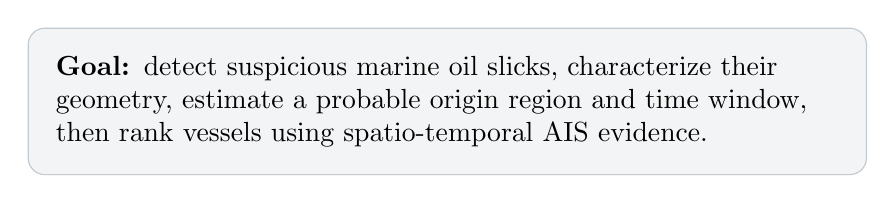
\begin{tikzpicture}
\node[rounded corners=6pt,fill=navy!5,draw=navy!25,
inner sep=10pt,text width=0.82\textwidth,align=left]{
\textbf{Goal:} detect suspicious marine oil slicks, characterize their geometry,
estimate a probable origin region and time window, then rank vessels using
spatio-temporal AIS evidence.
};
\end{tikzpicture}

\vfill
\large\textbf{Problem Statement 26143}
\hfill
\large Review 1
\end{frame}

% 2
\begin{frame}[t]{01 \quad Problem and objective}
\small
\textbf{\color{navy}The problem has two levels: detection and investigation.}

\vspace{0.15cm}
\begin{columns}[T,totalwidth=\textwidth]
\column{0.48\textwidth}
\textbf{\color{blue}What must be detected?}
\begin{itemize}
\item Suspicious oil-like surface signatures in satellite SAR.
\item Slick location, shape, extent and confidence.
\item Oil versus common SAR look-alikes.
\end{itemize}

\column{0.48\textwidth}
\textbf{\color{red}What must be inferred?}
\begin{itemize}
\item Where the slick could have originated.
\item When the release could have occurred.
\item Which vessels were consistent with that origin.
\end{itemize}
\end{columns}

\vspace{0.3cm}
\begin{center}
\pill{blue}{DETECT} \quad $\rightarrow$ \quad
\pill{teal}{CHARACTERIZE} \quad $\rightarrow$ \quad
\pill{orange}{BACKTRACK} \quad $\rightarrow$ \quad
\pill{red}{RANK VESSELS}
\end{center}

\vspace{0.25cm}
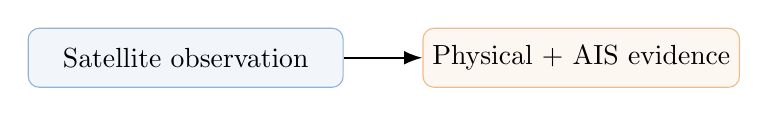
\begin{tikzpicture}
\node[draw=blue!50,fill=blue!6,rounded corners,minimum width=4.0cm,
minimum height=0.75cm,align=center] (a){Satellite observation};
\node[right=1.0cm of a,draw=orange!50,fill=orange!6,rounded corners,
minimum width=4.0cm,minimum height=0.75cm,align=center] (b){Physical + AIS evidence};
\draw[-{Latex},thick] (a)--(b);
\end{tikzpicture}

\vspace{0.15cm}
\textbf{Important:} the system ranks candidates. It does not declare legal culpability.
\end{frame}

% 3
\begin{frame}[t]{02 \quad Scientific basis: why SAR detects oil-like patterns}
\small
\begin{columns}[T,totalwidth=\textwidth]
\column{0.48\textwidth}
\textbf{\color{blue}Sentinel-1 SAR}
\begin{itemize}
\item Active microwave imaging works day and night and through cloud cover.
\item SAR measures returned radar backscatter from the sea surface.
\item Ocean backscatter depends strongly on surface roughness.
\item Oil films can damp small surface waves.
\item Reduced roughness can produce a darker SAR signature.
\end{itemize}

\column{0.47\textwidth}
\textbf{\color{red}The key limitation}
\begin{center}
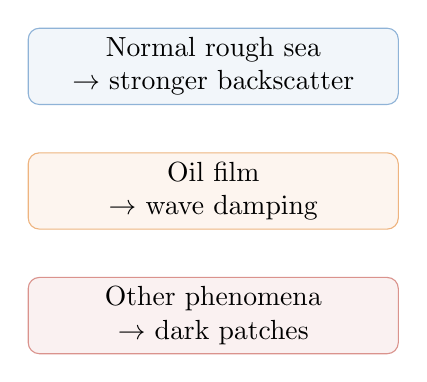
\begin{tikzpicture}[node distance=6mm]
\node[draw=blue!50,fill=blue!6,rounded corners,minimum width=4.7cm,
minimum height=0.8cm,align=center] (n)
{Normal rough sea\\$\rightarrow$ stronger backscatter};
\node[below=of n,draw=orange!55,fill=orange!7,rounded corners,
minimum width=4.7cm,minimum height=0.8cm,align=center] (o)
{Oil film\\$\rightarrow$ wave damping};
\node[below=of o,draw=red!55,fill=red!7,rounded corners,
minimum width=4.7cm,minimum height=0.8cm,align=center] (l)
{Other phenomena\\$\rightarrow$ dark patches};
\end{tikzpicture}
\end{center}

\vspace{0.15cm}
\begin{center}
{\Large\bfseries\color{red}Dark SAR patch $\neq$ automatically oil}
\end{center}
\end{columns}

\vspace{0.2cm}
\scriptsize\color{midgray}SAR provides an indirect surface signature. It does not directly identify chemical composition.
\end{frame}

% 4
\begin{frame}[t]{03 \quad Existing approaches and why DL is needed}\scriptsize
\small
\begin{columns}[T,totalwidth=\textwidth]
\column{0.31\textwidth}
\textbf{\color{gray}Traditional}
\begin{itemize}
\item Visual interpretation.
\item Intensity or threshold rules.
\item Manual polygon extraction.
\end{itemize}
\textbf{Weakness}
\begin{itemize}
\item Sensitive to imaging conditions.
\item Difficult to scale.
\item High false positives.
\end{itemize}

\column{0.31\textwidth}
\textbf{\color{blue}Deep learning}
\begin{itemize}
\item Learns spatial context.
\item Uses texture, shape and polarization.
\item Produces pixel-level masks.
\end{itemize}
\textbf{Weakness}
\begin{itemize}
\item Needs representative labels.
\item Can suffer from domain shift.
\end{itemize}

\column{0.31\textwidth}
\textbf{\color{teal}Operational attribution}
\begin{itemize}
\item AIS gives vessel trajectories.
\item Drift models constrain possible origins.
\item Combining both gives physical evidence.
\end{itemize}
\textbf{Remaining gap}
\begin{itemize}
\item Detection alone does not identify a source.
\item Nearest-vessel matching ignores drift and time.
\end{itemize}
\end{columns}

\vspace{0.25cm}
\begin{center}
\pill{red}{Core gap} \quad
\textbf{Connect image evidence to physical origin and vessel history.}
\end{center}
\vspace{-0.18cm}
\vspace{-0.28cm}
\end{frame}

% 5
\begin{frame}[t]{04 \quad Proposed solution}
\vspace{0.05cm}
\begin{center}

{\fontsize{20}{34}\selectfont\bfseries\color{navy}
DETECT $\rightarrow$ CHARACTERIZE $\rightarrow$ BACKTRACK}
\\[0.2cm]
{\fontsize{20}{34}\selectfont\bfseries\color{navy}
$\rightarrow$ CORRELATE $\rightarrow$ RANK}
\end{center}

\vspace{0.25cm}
\begin{center}
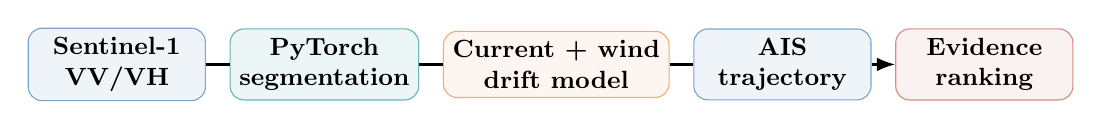
\begin{tikzpicture}[node distance=3mm]
\tikzstyle{B}=[draw,rounded corners=5pt,minimum width=2.25cm,
minimum height=0.82cm,align=center,font=\bfseries\small]
\node[B,draw=blue!60,fill=blue!7] (a){Sentinel-1\\VV/VH};
\node[B,draw=teal!60,fill=teal!7,right=of a] (b){PyTorch\\segmentation};
\node[B,draw=orange!60,fill=orange!7,right=of b] (c){Current + wind\\drift model};
\node[B,draw=blue!60,fill=blue!7,right=of c] (d){AIS\\trajectory};
\node[B,draw=red!60,fill=red!7,right=of d] (e){Evidence\\ranking};
\draw[-{Latex},thick] (a)--(b)--(c)--(d)--(e);
\end{tikzpicture}
\end{center}

\vspace{0.3cm}
\begin{columns}[T,totalwidth=\textwidth]
\column{0.31\textwidth}
\centering\textbf{\color{blue}AI layer}\\
Oil / look-alike classification and slick segmentation.

\column{0.31\textwidth}
\centering\textbf{\color{orange}Physics layer}\\
Backward particle trajectories estimate possible origins.

\column{0.31\textwidth}
\centering\textbf{\color{red}Evidence layer}\\
AIS space-time consistency produces candidate scores.
\end{columns}
\end{frame}

% 6
\begin{frame}[t]{05 \quad What exactly do we detect?}
\small
\begin{columns}[T,totalwidth=\textwidth]
\column{0.30\textwidth}
\begin{center}
\pill{blue}{OIL SLICK}
\end{center}
\begin{itemize}
\item Oil-like SAR signature.
\item Pixel mask.
\item Area, centroid, perimeter.
\item Orientation and elongation.
\end{itemize}

\column{0.30\textwidth}
\begin{center}
\pill{orange}{LOOK-ALIKE}
\end{center}
\begin{itemize}
\item Low-wind areas.
\item Biogenic films.
\item Rain-related effects.
\item Internal waves and wakes.
\end{itemize}

\column{0.30\textwidth}
\begin{center}
\pill{teal}{NO OIL}
\end{center}
\begin{itemize}
\item Normal ocean background.
\item Prevents ``dark = oil'' learning.
\item Supports false-positive control.
\end{itemize}
\end{columns}

\vspace{0.25cm}
\begin{center}
\[
\boxed{\text{SAR patch} \rightarrow
\text{Oil probability} + \text{Segmentation mask} + \text{Confidence}}
\]
\end{center}

\vspace{0.15cm}
\textbf{Why DL?} The model learns context, texture, shape and multi-channel patterns
that a single intensity threshold cannot represent.
\end{frame}

% 7
\begin{frame}[t]{06 \quad Three data streams}
\scriptsize
\renewcommand{\arraystretch}{1.35}
\begin{tabular}{>{\bfseries}p{2.15cm} p{3.65cm} p{3.7cm} p{2.65cm}}
\toprule
Data & What it gives & Acquisition & Role\\
\midrule
Sentinel-1 SAR &
VV/VH backscatter, metadata, oil masks &
Public Sentinel-1 products and research datasets &
Detection + geometry\\
AIS &
MMSI, timestamp, latitude, longitude, SOG, COG, vessel metadata &
MarineCadastre or another permitted AIS source &
Vessel history\\
Ocean + wind &
Surface current vectors and wind forcing &
Copernicus Marine + ERA5 or equivalent &
Drift simulation\\
\bottomrule
\end{tabular}

\vspace{0.25cm}
\begin{center}
\pill{blue}{OBSERVE} \quad+\quad
\pill{orange}{MODEL MOVEMENT} \quad+\quad
\pill{teal}{RECONSTRUCT VESSELS}
\end{center}

\vspace{0.2cm}
\textbf{Alignment:} use one coordinate system and UTC timestamps across all streams.
\end{frame}

% 8
\begin{frame}[t]{07 \quad Dataset details and how we use them}
\small
\begin{columns}[T,totalwidth=\textwidth]
\column{0.48\textwidth}
\textbf{\color{blue}Sentinel-1 oil-spill benchmark}
\begin{itemize}
\item Oil-spill images with corresponding segmentation masks.
\item VV/VH SAR channels in the benchmark release.
\item Separate material for oil, no-oil and look-alike discrimination.
\item Held-out test material supports unbiased evaluation.
\end{itemize}

\vspace{0.15cm}
\textbf{Use:}
\[
\text{Train} \rightarrow \text{Validate} \rightarrow \text{Test}
\]

\column{0.48\textwidth}
\textbf{\color{orange}AIS dataset}
\begin{itemize}
\item Vessel identity through MMSI.
\item Time-stamped position history.
\item Speed and course.
\item Vessel metadata where available.
\end{itemize}

\vspace{0.15cm}
\textbf{\color{teal}Environmental data}
\begin{itemize}
\item Current vector field.
\item Wind vector field.
\item Interpolated to the simulation time and location.
\end{itemize}
\end{columns}

\vspace{0.2cm}
\end{frame}

% 9
\begin{frame}[t]{08 \quad Preprocessing and model training}
\small
\begin{columns}[T,totalwidth=\textwidth]
\column{0.47\textwidth}
\textbf{\color{blue}SAR preprocessing}
\begin{enumerate}
\item Validate scene metadata.
\item Select VV/VH channels.
\item Normalize consistently.
\item Tile large scenes.
\item Keep image-mask alignment.
\item Augment training data only.
\end{enumerate}

\column{0.47\textwidth}
\textbf{\color{teal}Training setup}
\begin{enumerate}
\item PyTorch Dataset and DataLoader.
\item Train / validation / test separation.
\item U-Net baseline for segmentation.
\item BCE + Dice loss.
\item Save best validation checkpoint.
\item Evaluate only once on held-out test data.
\end{enumerate}
\end{columns}

\vspace{0.25cm}
\begin{center}
\pill{red}{Prevent leakage}
\quad
\pill{blue}{Preserve geospatial alignment}
\quad
\pill{teal}{Keep test data untouched}
\end{center}
\end{frame}

% 10
\begin{frame}[t]{09 \quad Deep-learning model: PyTorch U-Net baseline}
\small
\begin{columns}[T,totalwidth=\textwidth]
\column{0.56\textwidth}
\textbf{\color{blue}Input}
\begin{itemize}
\item SAR patch, typically VV + VH.
\item Fixed-size training tiles.
\end{itemize}

\textbf{\color{teal}Network}
\begin{itemize}
\item Encoder extracts hierarchical features.
\item Bottleneck captures high-level context.
\item Decoder restores spatial resolution.
\item Skip connections preserve slick boundaries.
\end{itemize}

\textbf{\color{orange}Output}
\begin{itemize}
\item Pixel-level oil probability map.
\item Thresholded segmentation mask.
\end{itemize}

\column{0.38\textwidth}
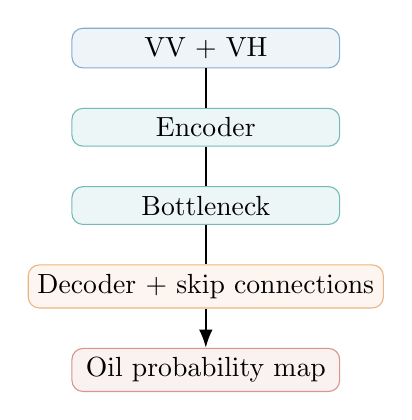
\begin{tikzpicture}[node distance=5mm]
\node[draw=blue!55,fill=blue!7,rounded corners,minimum width=3.4cm,
minimum height=0.48cm] (i){VV + VH};
\node[below=of i,draw=teal!55,fill=teal!7,rounded corners,minimum width=3.4cm,
minimum height=0.48cm] (e){Encoder};
\node[below=of e,draw=teal!55,fill=teal!7,rounded corners,minimum width=3.4cm,
minimum height=0.48cm] (b){Bottleneck};
\node[below=of b,draw=orange!55,fill=orange!7,rounded corners,minimum width=3.4cm,
minimum height=0.48cm] (d){Decoder + skip connections};
\node[below=of d,draw=red!55,fill=red!7,rounded corners,minimum width=3.4cm,
minimum height=0.48cm] (o){Oil probability map};
\draw[-{Latex},thick] (i)--(e)--(b)--(d)--(o);
\end{tikzpicture}
\end{columns}

\vspace{0.0cm}
\scriptsize\[
\mathcal{L}=\lambda_1\mathcal{L}_{BCE}+\lambda_2\mathcal{L}_{Dice}
\]
\vspace{-0.18cm}
\vspace{-0.25cm}
\end{frame}

% 11
\begin{frame}[t]{10 \quad Backtracking: estimating the probable origin}\footnotesize
\small
\textbf{Core idea:} start from the observed slick and integrate representative
particles backward through the environmental field.

\vspace{0.15cm}
\begin{center}
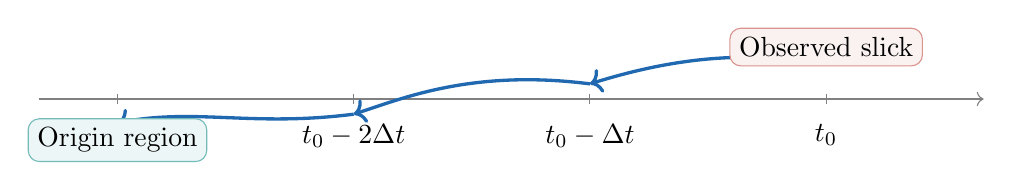
\begin{tikzpicture}[x=1cm,y=0.55cm]
\draw[->,gray] (0,0)--(12,0);
\foreach \x/\lab in {1/$t_0-3\Delta t$,4/$t_0-2\Delta t$,7/$t_0-\Delta t$,10/$t_0$}{
\draw[gray] (\x,-0.12)--(\x,0.12);
\node[below=2mm] at (\x,0){\lab};
}
\draw[blue,very thick,->] (10,0.8)..controls(8.8,1.2)and(7.8,0.8)..(7,0.35);
\draw[blue,very thick,->] (7,0.35)..controls(5.5,0.7)and(4.6,0.0)..(4,-0.35);
\draw[blue,very thick,->] (4,-0.35)..controls(2.7,-0.65)and(2.0,-0.2)..(1,-0.55);
\node[draw=red!55,fill=red!7,rounded corners] at (10,1.2){Observed slick};
\node[draw=teal!55,fill=teal!7,rounded corners] at (1,-0.95){Origin region};
\end{tikzpicture}
\end{center}

\vspace{0.1cm}
\[
\frac{d\mathbf{x}}{dt}
=
\mathbf{u}_{current}(\mathbf{x},t)
+
\alpha\,\mathbf{u}_{wind}(\mathbf{x},t)
+
\boldsymbol{\epsilon}
\]

\begin{itemize}
\item Use a Lagrangian particle model, such as OpenDrift, or a validated custom implementation.
\item Run backward trajectories to estimate an origin probability region.
\item Run forward trajectories to support short-term slick forecasting.
\end{itemize}

\textbf{\color{red}Output:} a probable origin distribution, not an exact historical point.
\end{frame}

% 12
\begin{frame}[t]{11 \quad AIS correlation and vessel ranking}
\footnotesize
\begin{columns}[T,totalwidth=\textwidth]
\column{0.47\textwidth}
\textbf{1. Spatial filter}
\begin{itemize}
\item Find vessels near the origin uncertainty region.
\item Keep a configurable search radius.
\end{itemize}

\textbf{2. Temporal filter}
\begin{itemize}
\item Compare vessel presence with the estimated release window.
\item Reconstruct the vessel trajectory around that window.
\end{itemize}

\textbf{3. Physical consistency}
\begin{itemize}
\item Check whether the observed slick could drift from the candidate location to the observed location.
\end{itemize}

\column{0.47\textwidth}
\textbf{Evidence score}
{\scriptsize
\[
S_v=w_sS_{space}+w_tS_{time}+w_dS_{drift}+w_bS_{behavior}
\]
}

\begin{itemize}
\item Spatial proximity to origin.
\item Temporal compatibility.
\item Drift consistency.
\item Optional behavior anomalies.
\end{itemize}

\vspace{0.05cm}
\begin{center}\normalsize\bfseries\color{red}Rank candidates, do not accuse automatically.\end{center}
\end{columns}
\end{frame}

% 13
\begin{frame}[t]{12 \quad System architecture and technology stack}
\small
\begin{center}
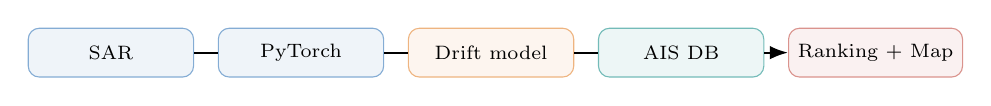
\begin{tikzpicture}[node distance=3mm]
\tikzstyle{B}=[draw,rounded corners=4pt,minimum width=2.1cm,
minimum height=0.62cm,align=center,font=\scriptsize]
\node[B,draw=blue!55,fill=blue!7](a){SAR};
\node[B,draw=blue!55,fill=blue!7,right=of a](b){PyTorch};
\node[B,draw=orange!55,fill=orange!7,right=of b](c){Drift model};
\node[B,draw=teal!55,fill=teal!7,right=of c](d){AIS DB};
\node[B,draw=red!55,fill=red!7,right=of d](e){Ranking + Map};
\draw[-{Latex},thick](a)--(b)--(c)--(d)--(e);
\end{tikzpicture}
\end{center}

\vspace{0.2cm}
\begin{columns}[T,totalwidth=\textwidth]
\column{0.31\textwidth}
\textbf{\color{blue}ML / CV}
\begin{itemize}
\item Python
\item PyTorch
\item NumPy
\item OpenCV
\item scikit-learn
\end{itemize}

\column{0.31\textwidth}
\textbf{\color{teal}Geospatial}
\begin{itemize}
\item Rasterio
\item GeoPandas
\item Shapely
\item xarray
\item OpenDrift
\end{itemize}

\column{0.31\textwidth}
\textbf{\color{orange}Backend / UI}
\begin{itemize}
\item FastAPI
\item PostgreSQL + PostGIS
\item React
\item Leaflet / MapLibre
\item Docker
\end{itemize}
\end{columns}

\vspace{0.2cm}
\textbf{Prototype principle:} each module produces inspectable outputs for the next module.
\end{frame}

% 14
\begin{frame}[t]{13 \quad Novelty, validation and feasibility}
\small
\begin{columns}[T,totalwidth=\textwidth]
\column{0.47\textwidth}
\textbf{\color{red}Novelty}
\begin{enumerate}
\item Explicit oil versus look-alike learning.
\item Physics-informed origin estimation.
\item Backward + forward slick reasoning.
\item Spatio-temporal AIS candidate scoring.
\item Evidence display instead of black-box accusation.
\end{enumerate}

\column{0.47\textwidth}
\textbf{\color{blue}Validation}
\begin{itemize}
\item Segmentation: IoU, Dice, precision, recall.
\item Origin: localization error in km.
\item Time: origin-time error.
\item Attribution: Top-1 / Top-k recovery on controlled cases.
\end{itemize}

\vspace{0.1cm}
\textbf{\color{green}Feasibility}
\begin{itemize}
\item Public research data can support the prototype.
\item Open-source ML and geospatial tools.
\item Main compute need is model training.
\end{itemize}
\end{columns}

\vspace{0.12cm}
\begin{center}\pill{red}{Novelty} \quad
\pill{blue}{Measurable} \quad
\pill{green}{Low-cost prototype}
\end{center}
\vspace{-0.18cm}
\end{frame}



\end{document}

